\documentclass{acaces}


%%%%%%%%%%%%%%%%%%%%%%%%%
%% Document and Layout %%
%%%%%%%%%%%%%%%%%%%%%%%%%

% Fix for multiple "No room for a new \dimen" errors.
%
% See: http://tex.stackexchange.com/questions/38607/no-room-for-a-new-dimen
%
\usepackage{etex}

% Fix for "'babel/polyglossia' detected but 'csquotes' missing"
% warning. NOTE: Include after inputenc.
%
\usepackage{csquotes}
\usepackage{booktabs}

% Required for full page-width tables.
\usepackage{tabularx}

\usepackage{wrapfig}

\usepackage{adjustbox}

% Define column types L, C, R with known text justification and fixed
% widths:
\usepackage{array}
\newcolumntype{L}[1]{>{\raggedright\let\newline\\\arraybackslash\hspace{0pt}}m{#1}}
\newcolumntype{C}[1]{>{\centering\let\newline\\\arraybackslash\hspace{0pt}}m{#1}}
\newcolumntype{R}[1]{>{\raggedleft\let\newline\\\arraybackslash\hspace{0pt}}m{#1}}

% Make internal macro definitions accessible,
% e.g. \@title, \@date \@author.
\makeatletter

%%%%%%%%%%%%%%%%%%%%%
% Table of Contents %
%%%%%%%%%%%%%%%%%%%%%

\usepackage{color}
\newcommand{\fix}[1]{\textcolor{red}{\em\footnotesize#1}}


%%%%%%%%%%%%%%%%
% Bibliography %
%%%%%%%%%%%%%%%%
\usepackage[%
    backend=biber,%bibtex,
    style=numeric-comp,
    % style=numeric-comp,  % numerical-compressed
    sorting=none,        % nty,nyt,nyvt,anyt,anyvt,ynt,ydnt,none
    sortcites=true,      % sort \cite{b a d c}: true,false
    block=none,          % space between blocks: none,space,par,nbpar,ragged
    indexing=false,      % indexing options: true,false,cite,bib
    citereset=none,      % don't reset cites
    isbn=false,          % print ISBN?
    url=true,            % print URL?
    doi=false,           % print DOI?
    natbib=true,         % natbib compatability
    maxbibnames=99       % no 'et-al' in the bibliography pls
  ]{biblatex}

\addbibresource{../../../library.bib}

% Reduce the font size of the bibliography:
\renewcommand{\bibfont}{\normalfont\scriptsize}

\usepackage{setspace}
\onehalfspacing


%%%%%%%%%%%%%%%%%%%%%%%%%%%%%%%%%%%%%
%% Figures, footnotes and listings %%
%%%%%%%%%%%%%%%%%%%%%%%%%%%%%%%%%%%%%

% Pre-requisites for rendering upquotes in listings package.
\usepackage[T1]{fontenc}
\usepackage{lmodern}
\usepackage{textcomp}

% Pseudo-code listings.
\usepackage{algorithm}
\usepackage{algpseudocode}
\newcommand{\Break}{\State \textbf{break} }
\algblockdefx[Loop]{Loop}{EndLoop}[1][]{\textbf{Loop} #1}{\textbf{End
    Loop}}

\algrenewcommand\ALG@beginalgorithmic{\footnotesize}


%%%%%%%%%%%%%%%%%%%%%%%%
%% Graphics and maths %%
%%%%%%%%%%%%%%%%%%%%%%%%
\usepackage{amsmath}

% Vector notation, e.g. \vv{x}:
%
\usepackage{esvect}

% Additional amsmath symbols, see:
%
% http://texblog.org/2007/08/27/number-sets-prime-natural-integer-rational-real-and-complex-in-latex/
%
\usepackage{amsfonts}
\usepackage{amssymb}

\usepackage{graphicx}
\usepackage{mathtools}

% Provide bold font face in maths.
\usepackage{bm}

\usepackage{subcaption}
\expandafter\def\csname ver@subfig.sty\endcsname{}

% Define an 'myalignat' command which behave as 'alignat' without the
% vertical top and bottom padding. See:
%     http://www.latex-community.org/forum/viewtopic.php?f=5&t=1890
\newenvironment{myalignat}[1]{%
  \setlength{\abovedisplayskip}{-.7\baselineskip}%
  \setlength{\abovedisplayshortskip}{\abovedisplayskip}%
  \start@align\z@\st@rredtrue#1
}%
{\endalign}

% Define additional operators:
\DeclareMathOperator*{\argmin}{arg\,min}
\DeclareMathOperator*{\argmax}{arg\,max}

\DeclareMathOperator*{\gain}{Gain}

% Skeleton operators.
\DeclareMathOperator*{\map}{Map}
\DeclareMathOperator*{\reduce}{Reduce}
\DeclareMathOperator*{\scan}{Scan}
\DeclareMathOperator*{\stencil}{Stencil}
\DeclareMathOperator*{\zip}{Zip}
\DeclareMathOperator*{\allpairs}{All\,Pairs}

% Define a command to allow word breaking.
\newcommand*\wrapletters[1]{\wr@pletters#1\@nil}
\def\wr@pletters#1#2\@nil{#1\allowbreak\if&#2&\else\wr@pletters#2\@nil\fi}

% Define a command to create centred page titles.
\newcommand{\centredtitle}[1]{
  \begin{center}
    \large
    \vspace{0.9cm}
    \textbf{#1}
  \end{center}}

% Provide generic commands \degree, \celsius, \perthousand, \micro
% and \ohm which work both in text and maths mode.
\usepackage{gensymb}

\begin{document}

\title{Autotuning OpenCL Workgroup Sizes}

\author{
Chris~Cummins\addressnum{1},
Pavlos~Petoumenos\addressnum{1},
Michel~Steuwer\addressnum{1},
Hugh~Leather\addressnum{1}
}

\address{1}{
University of Edinburgh,
UK
}

\extra{1}{% Contacts
  E-mail: c.cummins@ed.ac.uk, ppetoume@inf.ed.ac.uk,
  michel.steuwer@ed.ac.uk, hleather@inf.ed.ac.uk%
}%
\extra{2}{% Acknowledgements
  This work was supported by the UK EPSRC under grants EP/L01503X/1
  (CDT in Pervasive Parallelism), EP/H044752/1 (ALEA), and
  EP/M015793/1 (DIVIDEND).%
}

\pagestyle{empty}


\begin{abstract}
  Selecting appropriate workgroup sizes for OpenCL programs is
  critical for performance, and requires knowledge of the underlying
  hardware, the data being operated on, and the behaviour of the
  kernel. Ensuring performance portability of OpenCL programs is
  challenging, since simple heuristics and statically chosen values
  fail to exploit the available performance. To address this, we
  propose the use of machine learning-enabled autotuning to
  automatically predict workgroup sizes for stencil patterns on CPUs
  and multi-GPUs. We present three methodologies for predicting OpenCL
  workgroup sizes, and evaluate the effectiveness of each in a study
  of 429 combinations of architecture, kernel, and dataset. We compare
  an average of 629 different workgroup sizes for each case, finding
  that autotuning provides a median $3.79\times$ speedup over the best
  possible fixed workgroup size, achieving 94\% of the maximum
  performance.
\end{abstract}

\vspace{-.5em}
\keywords{%
  OpenCL; %
  Autotuning; %
  Stencils; %
  GPUs; %
  Machine learning; %
  Synthetic benchmarking%
}

\vspace{-2em}
\section{Introduction}

Efficient, tuned implementations of stencil codes are highly sought
after, with a variety of applications from fluid dynamics to quantum
mechanics. OpenCL enables the application of a range of heterogeneous
devices to parallelise stencils; however, achieving portable
performance is a hard task --- OpenCL kernels are sensitive to
properties of the underlying hardware, to the implementation, and even
to the dataset that is operated upon. This forces developers to
laboriously hand tune performance on a case-by-case basis, since
simple heuristics fail to exploit the available performance. In this
work we demonstrate how machine learning-enabled autotuning can be
applied to Algorithmic Skeletons to achieve near optimal performance
of stencils operations, without requiring hand tuning.

\begin{wrapfigure}{r}{0.38\textwidth}
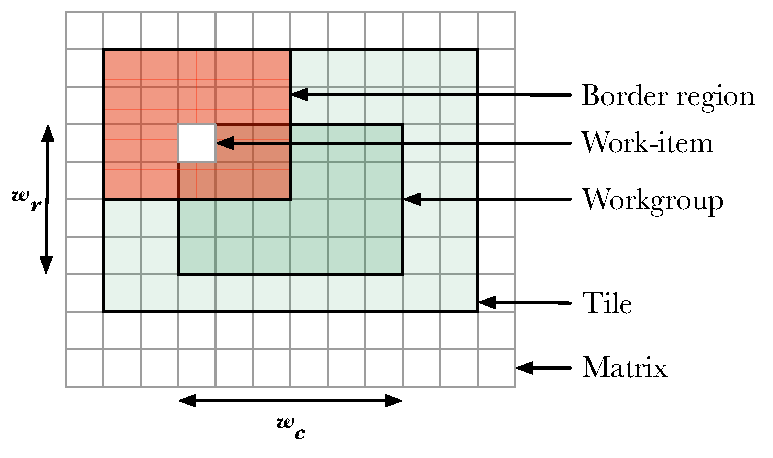
\includegraphics[width=.38\textwidth]{stencil}
\caption[Stencil border region]{%
  The components of a stencil: an input matrix is decomposed into
  workgroups, and elements within workgroups are mapped to work-items.
  The values used by workgroups are mapped to local memory.%
  \vspace{-.75em} }
\label{fig:stencil-shape}
\end{wrapfigure}

SkelCL is an Algorithmic Skeleton library which provides OpenCL
implementations of data parallel patterns for heterogeneous
parallelism using CPUs and
multi-GPUs~\cite{Steuwer2011}. Figure~\ref{fig:stencil-shape} shows
the components of the SkelCL stencil pattern, which applies a
user-provided \emph{customising function} to each element of a 2D
matrix. The value of each element is updated based on its current
value and the value of one or more neighbouring elements, called the
\emph{border region}. When a SkelCL stencil pattern is executed, each
of the matrix elements are mapped to OpenCL work-items; and this
collection of work-items is divided into \emph{workgroups} for
execution on the target hardware. A \emph{tile} of elements the size
of the workgroup and the perimeter border region is allocated in local
memory for use by work-items. Changing the workgroup size affects both
the number of workgroups which can be active simultaneously, and the
amount of local memory required for each workgroup. While the user
defines the size, type, and border region of the matrix being operated
upon, it is the responsibility of the SkelCL implementation to select
an appropriate workgroup size to use.

\section{Autotuning OpenCL Workgroup Size}

Selecting an appropriate workgroup size $w$ depends on the properties
of kernel, hardware, and dataset, as illustrated in
Figures~\ref{fig:motivation-arch} and~\ref{fig:motivation-prog}. The
workgroup size space $W$ is subject to hard constraints which cannot
conveniently be statically determined. Each OpenCL device and kernel
imposes a maximum workgroup size, determined by the hardware resources
and resource requirements of a program. Additionally, not all points
in the workgroup size space are found to provide correct programs. A
\emph{refused parameter} is a workgroup size which satisfies the
kernel and architectural constraints, yet causes a
\texttt{CL\_OUT\_OF\_RESOURCES} error to be thrown when the kernel is
enqueued (in many OpenCL implementations this is a generic error code
and may not necessarily indicate that a finite resource
constraint). We define a \emph{legal} workgroup size as one which, for
a given \emph{scenario} $s$ (a combination of program, device, and
dataset), satisfies the architectural and kernel constraints, and is
not refused. The subset of all possible workgroup sizes
$W_{legal}(s) \subset W$ that are legal for a given scenario $s$ is
then:
%
\begin{equation}
  W_{legal}(s) = \left\{w | w \in W, w < W_{\max}(s) \right\} - W_{refused}(s)
\end{equation}
%
Where $W_{\max}(s)$ can be determined at runtime prior to the kernels
execution, but the set $W_{refused}(s)$ can only be determined
experimentally.


\begin{figure}
\centering
\adjustbox{valign=t}{%
  \begin{minipage}{.48\textwidth}
    \centering
    \begin{subfigure}[h]{.48\columnwidth}
      \centering
      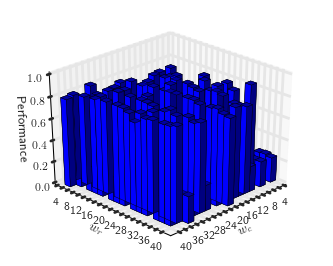
\includegraphics[width=1.0\columnwidth]{motivation_1}
      \vspace{-1.5em} % Shrink vertical padding
      \caption{}
      \label{fig:motivation-1}
    \end{subfigure}
    ~%
    \begin{subfigure}[h]{.48\columnwidth}
      \centering
      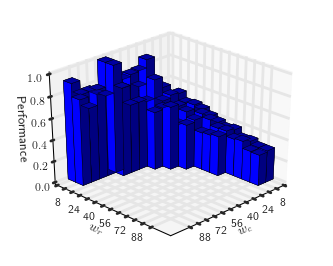
\includegraphics[width=1.0\columnwidth]{motivation_2}
      \vspace{-1.5em} % Shrink vertical padding
      \caption{}
      \label{fig:motivation-2}
    \end{subfigure}
    \caption{%
      The performance of different workgroup sizes for the same
      stencil program on two different devices:
      (\subref{fig:motivation-1}) Intel CPU,
      (\subref{fig:motivation-2}) NVIDIA GPU.%
    }
    \label{fig:motivation-arch}
  \end{minipage}%
}%
\hspace{2.5mm}
\adjustbox{valign=t}{%
  \begin{minipage}{.48\textwidth}
    \centering
    \begin{subfigure}[h]{.48\columnwidth}
      \centering
      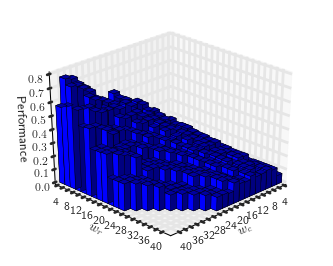
\includegraphics[width=1.0\columnwidth]{motivation_3}
      \vspace{-1.5em} % Shrink vertical padding
      \caption{}
      \label{fig:motivation-3}
    \end{subfigure}
    ~%
    \begin{subfigure}[h]{.48\columnwidth}
      \centering
      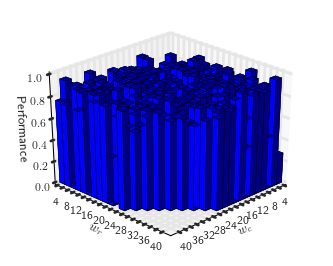
\includegraphics[width=1.0\columnwidth]{motivation_4}
      \vspace{-1.5em} % Shrink vertical padding
      \caption{}
      \label{fig:motivation-4}
    \end{subfigure}
    \caption{%
      The performance of different workgroup sizes for the same device
      executing two different stencil programs.%
    }
    \label{fig:motivation-prog}
  \end{minipage}%
}
\end{figure}


\subsection{Machine Learning Methods}\label{sec:ml}

The OpenCL workgroup size optimization space is large, complex, and
non-linear. Successfully applying machine learning to this space
requires plentiful training data, the careful selection of explanatory
variables, and appropriate machine learning methods. Our approach uses
a \textit{classifier} to automatically correlate patterns between
explanatory variables and the workgroup sizes which provide optimal
performance. The classifier used is the popular J48 Decision
Tree~\cite{Han2011}, chosen due to its low runtime cost and ability to
efficiently handle large dimensionality training data.

For each scenario, a total of 102 explanatory variables are extracted
to capture information about the device, program, and dataset. Device
variables encode the device type (e.g. CPU or GPU, integrated or
external, connection bus), properties about the host (e.g.\ system
memory, maximum clock frequency), and numerous properties about the
execution device (e.g.\ number of compute units, local memory size,
global caches). Program variables include instruction densities for
each instruction type, the total number of basic blocks, and the total
instruction count. They are extracted using static instruction count
passes over an LLVM IR compiled version of the user stencil
implementation. Dataset variables include the data types (input and
output), and dimensions of the input matrix and stencil region.

A parameterised template substitution engine is used to generate
synthetic stencil programs for generating training data. Stencil
templates are parameterised with a border region size and
\emph{complexity}, a simple metric to broadly dictate the number of
operations in a given stencil code. Once the performance of different
workgroup sizes for a scenario is assessed, the set of explanatory
variables describing the scenario is paired with the oracle workgroup
size. This process is repeated for multiple scenarios to create
training data. A classifier learns from this training data to make
predictions for new sets of explanatory variables, by predicting a
workgroup size from the set of oracle workgroup sizes of the training
data.

This approach presents the problem that there is no guarantee that the
set of workgroup sizes which may be predicted is within the set of
legal workgroup sizes for future scenarios. This may result in a
classifier predicting a workgroup size which is not legal for a
scenario, $w \not\in W_{legal}(s)$, either because it exceeds
$W_{\max}(s)$, or because the parameter is refused. If this occurs, a
\emph{nearest neighbor} approach is used to select the workgroup size
$w$ which is expected to be legal and has the lowest Euclidian
distance to the predicted value $c$. This is achieved by comparing row
($r$) and column ($c$) indices:
%
\begin{equation}
  w = \underset{w \in W_{legal(s)}}{\argmin} \sqrt{\left(c_r - w_r\right)^2 + \left(c_c - w_c\right)^2}
\end{equation}
%
This process of selecting alternative parameters will iterate until a
legal parameter is found.

\subsection{Evaluation Methodology}

An exhaustive enumeration of the workgroup size optimisation space for
429 combinations of architecture, program, and dataset was performed.
Seven architectures were used (3 NVIDIA GPUs, 3 Intel CPUs, and 1 AMD
GPU). Synthetically generated stencil programs and six reference
kernels taken from image processing, cellular automata, and partial
differential equation solving were used. Dataset sizes used were
$512\times512$, $1024\times1024$, $2048\times2048$, and
$4096\times4096$. The workgroup size space was enumerated for each
combination of $w_r$ and $w_c$ values in multiples of 2, up to the
maximum workgroup size. A minimum of 30 runtimes were recorded for
each scenario and the average execution time taken.

\section{Results}\label{sec:results}

\section{Conclusions}\label{sec:conclusions}

We present a novel methodology for autotuning the workgroup size of
stencil patterns using the established open source library
SkelCL. This technique achieves 94\% of the maximum performance, while
providing robust fallbacks in the presence of unexpected behaviour in
OpenCL driver implementations. In future work we will use machine
learning to perform a directed search through the program space by
guiding the generation of synthetic benchmark programs.


\label{bibliography}

\begingroup
\setstretch{0.8}
\setlength\bibitemsep{1pt}
\printbibliography
\endgroup

\end{document}
